\documentclass[utf8, 12pt, a4paper, oneside]{article}
\usepackage[mathletters]{ucs}
\usepackage[utf8x,utf8]{inputenc}
\usepackage[T2A]{fontenc}
\usepackage[english,russian]{babel}
\usepackage{indentfirst}
\usepackage{ulem}
\usepackage{pifont}
\usepackage{amsmath}
\usepackage{amssymb}
\usepackage{csquotes}  
\usepackage{bbm}
\usepackage{dsfont}
\usepackage{wasysym}
\usepackage{color}
\usepackage[usenames]{xcolor}
\usepackage{graphicx}
\usepackage{setspace}
\usepackage{xcolor}
\usepackage{hyperref}
\usepackage{pdfpages}
\definecolor{linkcolor}{HTML}{799B03} % цвет ссылок
\definecolor{urlcolor}{HTML}{799B03} % цвет гиперссылок
\hypersetup{pdfstartview=FitH,  linkcolor=linkcolor,urlcolor=urlcolor, colorlinks=true}
\usepackage{verbatim}
\usepackage{shortvrb}
\usepackage[overload]{empheq}
\usepackage{listings}
 
 % Цвета для гиперссылок
\definecolor{linkcolor}{HTML}{799B03} % цвет ссылок
\definecolor{urlcolor}{HTML}{799B03} % цвет гиперссылок
 
\hypersetup{pdfstartview=FitH,  linkcolor=linkcolor,urlcolor=urlcolor, colorlinks=true}

    \lstset{
        language=C,                             % Code langugage
        tabsize=4,
        breaklines,
        columns=fullflexible,
        flexiblecolumns,
        frame=tb ,
        numbers=left,
        numberstyle=\footnotesize\color{brown!50},
        extendedchars = false,
        inputencoding = utf8,
        keepspaces = true,
        belowcaptionskip=5pt
    }

    %% Основной стиль
    \lstset{
        basicstyle=\ttfamily\small\color[rgb]{0.0,0.0,0},
    }

    %% Комментарии
    \lstset{
        commentstyle=\color[rgb]{0,0.5,0}\itshape,
    }

    %% Ключевые слова
    \lstset{
        keywordstyle=\bfseries\color{blue},
    }

    %% Строки
    \lstset{
        stringstyle=\ttfamily\color{gray},
        morestring=[b]",
        morestring=[d]
    }

    %% Цифры
    \lstset{literate=%
        {0}{{{\color{red}0}}}1
        {1}{{{\color{red}1}}}1
        {2}{{{\color{red}2}}}1
        {3}{{{\color{red}3}}}1
        {4}{{{\color{red}4}}}1
        {5}{{{\color{red}5}}}1
        {6}{{{\color{red}6}}}1
        {7}{{{\color{red}7}}}1
        {8}{{{\color{red}8}}}1
        {9}{{{\color{red}9}}}1
    %% Константы
        {NULL}{{{\bf\color{red!80!black}NULL}}}1
        {EOF}{{{\bf\color{red!80!black}EOF}}}1
    %% Операции
        {+}{{{\color{teal!50!black}+}}}1
        {-}{{{\color{teal!50!black}-}}}1
        {/}{{{\color{teal!50!black}/}}}1
        {*}{{{\color{teal!50!black}*}}}1
        {=}{{{\color{teal!50!black}=}}}1
        {\&}{{{\color{teal!50!black}\&}}}1
        {!}{{{\color{teal!50!black}!}}}1
        {==}{{{\color{orange!50!black}$==$}}}1
        {!=}{{{\color{orange!50!black}$!=$}}}1
        {++}{{{\color{red}$++$}}}1
        {--}{{{\color{red}$--$}}}1
    %% Свои вспомогательные типы
        {size\_t}{{{\color{teal}size\_t}}}1
        {surname\_t}{{{\color{teal}surname\_t}}}1
        {numberProc\_t}{{{\color{teal}numberProc\_t}}}1
        {typeProc\_t}{{{\color{teal}typeProc\_t}}}1
        {typeVideo\_t}{{{\color{teal}typeVideo\_t}}}1
        {typeVinchest\_t}{{{\color{teal}typeVinchest\_t}}}1
        {OS\_t}{{{\color{teal}OS\_t}}}1
        {comp\_t }{{{\color{teal}comp\_t }}}1
        {FILE}{{{\color{teal}FILE}}}1
    %% Стандартные вспомогательные функции
        {malloc}{{{\bf\color{violet!60!black}malloc}}}1
        {fgets}{{{\bf\color{violet!60!black}fgets}}}1
        {sscanf}{{{\bf\color{violet!60!black}sscanf}}}1
        {strcpy}{{{\bf\color{violet!60!black}strcpy}}}1
        {strlen}{{{\bf\color{violet!60!black}strlen}}}1
        {free}{{{\bf\color{violet!60!black}free}}}1
        {fopen}{{{\bf\color{violet!60!black}fopen}}}1
        {fflush}{{{\bf\color{violet!60!black}fflush}}}1
        {fclose}{{{\bf\color{violet!60!black}fclose}}}1
        {fread}{{{\bf\color{violet!60!black}fread}}}1
        {fwrite}{{{\bf\color{violet!60!black}fwrite}}}1
        {perror}{{{\bf\color{violet!60!black}fwrite}}}1
    }




\begin{document}
\thispagestyle{empty}

\begin{center}
Московский авиационный институт\\
\vspace{0.5cm}
Факультет прикладной математики и физики\\
\vspace{0.5cm}
Кафедра вычислительной математики и программирования\\

\vspace{3cm}

Лабораторная работа № 2\\
по дисциплине\\
"Численные методы"\\
\end{center}

\vspace{3cm}

\begin{flushright}
\begin{tabular}{rl}
Студент: & Балес А.И.\\
Преподаватель: & Ревизников Д.Л. \\
Дата: & \\
Оценка: & \\
Подпись: & \\
\end{tabular}
\end{flushright}

\vspace{5cm}

\begin{center}
Москва, 2016
\end{center}

\pagebreak

\subsection*{Постановка задачи:}
\parindent=1cm Необходимо реализовать алгоритм параллельного нахождения собственных значений и собственных векторов {\tt{методом вращений (Якоби)}}. Для решения данной проблемы можно пойти по одному из следующих путей:
\begin{itemize}
\item Путь наименьшего сопротивления -- распараллелить не сам алгоритм как таковой, а постараться распараллелить как можно больше его подчастей, т.е. перемножение матриц, транпспонирование матрицы, поиска максимального элемента в матрице. Данный способ менее эффективен чем тот, который будет описан в следующем пункте.
\item Постараться распараллелить не части алгоритма, а целиком направить вычисления на каждый процессор, а затем просто склеить значения воедино и все. Сложность представляется в том, что принцип разделения задачи на подзадачи не очевиден.
\end{itemize}

К сожалению, я пошел не по тому пути, по которому следовало бы... Давайте рассмотрим метод Якоби и попытаемся порассуждать о том, как можно было бы разбить на подзадачи данный агоритм.

\includepdf[pages={22-25}]{Part1.pdf}

Вот мои догадки по поводу того, как бы я решал эту задачу, разбивая алгоритм на подзадачи, которые бы решались параллельно, а затем решения склеивались бы в единую матрицу:
\begin{enumerate}
\item Первым делом в обычном методе Якоби ищется максимальный внедиагональный элемент, пусть его координаты будут $(m, l)$, где $m$--строка, а $l$--столбец, $\Rightarrow$ после умножения на матрицу вращения элемент $\mathbb{A}[m,l]$ и $\mathbb{A}[l,m]$ обнулятся (в силу симметричности).
\item После того, как выбрали элемент $\mathbb{A}[m,l]$ мы помечаем их как использованные, и в дальнейшем не будем выбирать ${m,l}$ как строки, так и столбцы. Т.е. дальнейший поиск максимумов будет осуществляться в строках и столбцах не равных ${m,l}$.
\item Для каждого из таких максимумов мы выделим по две строки ($m$ и $l$) и два столбца ($m$ и $l$) и будем осуществлять все операции только с ними. Следует быть осторожным с обработкой элементов, находящийхся на пересечении $m$ строки и $l$ столбца, а также $l$ строки и $m$ столбца, т.к. их нужно изменять в обоих массивах сразу.
\item Теперь сливаем все эти строки и столбцы снова в матрицу, и повторяешь п.1 пока не окажется, что все элементы в матрице $\{\mathbb{A}[i,j] | i \neq j\}  < \varepsilon$.
\end{enumerate}

\subsection*{Технологии:}
В настоящее время очень широкое применение имеют параллельные вычисления на GPU (графических процессорах), т.к. GPU более производительное, чем CPU. Обусловленно это тем, что GPU имеет огромное количество исполнительных блоков: в современных GPU их 2048 и более, в то время как у CPU их количество может достигать 48, но чаще всего их количество лежит в диапазоне 2-8. Есть множество различий и в поддержке многопоточности: CPU исполняет 1-2 потока вычислений на одно процессорное ядро, а GPU может поддерживать несколько тысяч потоков на каждый мультипроцессор, которых в чипе несколько штук! И если переключение с одного потока на другой для CPU стоит сотни тактов, то GPU переключает несколько потоков за один такт.

В CPU большая часть площади чипа занята под буферы команд, аппаратное предсказание ветвления и огромные объемы кэш-памяти, а в GPU большая часть площади занята исполнительными блоками. Вышеописанное устройство схематично изображено ниже:
\begin{center}
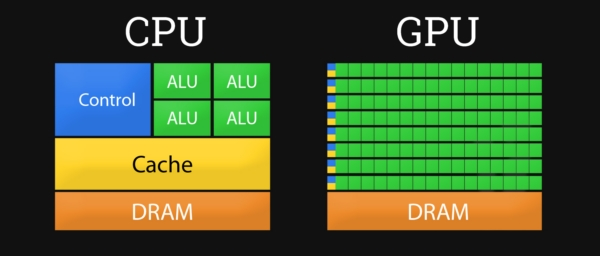
\includegraphics[scale=0.5]{compare_paper}
\end{center}

Если CPU -- это своего рода <<начальник>>, принимающий решения в соответствии с указаниями программы, то GPU -- это <<рабочий>>, который производит огромное количество однотипных вычислений. Выходит, что если подавать на GPU независимые простейшие математические задачи, то он справится значительно быстрее, чем центральный процессор.

Предлагаю теперь обсудить технологию, которой я пользовался при распараллеливании отдельных частей метода Якоби. Она называется {\tt{OpenCL}} (\textbf{Open} \textbf{C}omputing \textbf{L}anguage -- открытый язык вычислений) -- фреймворк для написания компьютерных программ, связанных с параллельными вычислениями на различных графических (GPU) и центральных процессорах (CPU), а также FPGA. Вo фреймворк OpenCL входят язык программирования, который базируется на стандарте C99, и интерфейс программирования приложений (API). OpenCL обеспечивает параллелизм на уровне инструкций и на уровне данных и является реализацией техники GPGPU. OpenCL является полностью открытым стандартом, его использование не облагается лицензионными отчислениями.

Цель OpenCL состоит в том, чтобы дополнить OpenGL и OpenAL, которые являются открытыми отраслевыми стандартами для трёхмерной компьютерной графики и звука, пользуясь возможностями GPU. OpenCL разрабатывается и поддерживается некоммерческим консорциумом \textit{Khronos Group}, в который входят много крупных компаний, включая \textsc{AMD, Apple, ARM, Intel, Nvidia, Sony Computer Entertainment, Sun Microsystems} и другие.

Если в кратце, то OpenCL кроссплатформенная технология распараллеливания вычислений на GPU $\Rightarrow$ без разницы, графический адаптер какой фирмы установлен на машине, будь то Nvidia или AMD, код на OpenCL будет выполняться аналогично на любых устройствах. В этом, несомненно, заключается его преимущество. Существует также и обратная сторона медали, для того, чтобы вызвать код на OpenCL необходимо сначала перенести все данные в буфер, с которым будет оперировать непосредственно процессор GPU. Время затрачиваемое на запись и считывание может существенно ухудшить показатели производительности, если нерационально применять распараллеливание на GPU.

Также стоит сказать и об альтернативной технологии -- CUDA, разработка компании Nvidia, которая в технологическом плане идет на шаг впереди OpenCL, но по сравнению с ней она является платформозависимой.

\subsection*{Алгоритм и реализация:}
В коде, который будет приведен ниже, происходит инициализация аппаратуры, а именно, происходит поиск платформ, далее на нужной платформе осуществляется поиск устройства, которое будет производить вычисления. После этого создается контекст и очередь задач. Контекст представляет собой пространство, в котором будут храниться все наши данные (буфферы). В очередь задач будут добавляться задачи на выполнение. Также нам потребуется создать кернелы, которые будет отвечать за отдельную функцию в коде на OpenCL, т.е. кернелы являются прослойкой между исходным кодом на C/C++ и кодом на OpenCL. Код на языке OpenCL компилируется в \textit{RUNTIME} режиме, его можно хранить как отдельным файлом, так и строкой внутри кода на C/C++.
\begin{lstlisting}
void RotateMethodGPU() {
    string plotFileGPU = "plotDataGPU";
    // инициализация устройств
    // ************************************************************************************
    cl_int              err;
    cl_platform_id*     platforms;
    cl_uint             num_platforms;
    cl_device_id*       devices;
    cl_uint             num_devices;
    cl_context          context;
    cl_command_queue    command_queue;
    cl_program          program                     = NULL;
    cl_kernel           kernelFindMaxAbs            = NULL;
    cl_kernel           kernelMultMatrix            = NULL;
    cl_kernel           kernelComputeNorm           = NULL;
    cl_kernel           kernelTranspose             = NULL;
    cl_context_properties platforms_properties[3];

    /* получить доступные платформы */
    err = clGetPlatformIDs(0, NULL, &num_platforms);
    checkRet(err, __LINE__);
    platforms = (cl_platform_id*)malloc(sizeof(cl_platform_id) * num_platforms);
    err = clGetPlatformIDs(num_platforms, platforms, NULL);
    checkRet(err, __LINE__);
    /* получить доступные устройства */
    // цикл нужен если платформ с GPU > 1
    //for (size_t i = 0; i < num_platforms; ++i) {
        platforms_properties[0] = (cl_context_properties)CL_CONTEXT_PLATFORM;  // indicates that next element is platform
        platforms_properties[1] = (cl_context_properties)platforms[0];  // platform is of type cl_platform_id
        platforms_properties[2] = (cl_context_properties)0;   // last element must b
        err = clGetDeviceIDs(platforms[0], CL_DEVICE_TYPE_GPU, 0, NULL, &num_devices);
        checkRet(err, __LINE__);
        devices = (cl_device_id*)malloc(sizeof(cl_device_id) * num_devices);
        err = clGetDeviceIDs(platforms[0], CL_DEVICE_TYPE_GPU, num_devices, devices, NULL);
        checkRet(err, __LINE__);
    //}
    size_t param_sz;
    cl_uint param_int, valFPS = 0;
    char* param_string;
    for (size_t i = 0; i < num_devices; ++i) {        
        err = clGetDeviceInfo(devices[i], CL_DEVICE_ADDRESS_BITS, sizeof(cl_uint), (void*)&param_int, NULL);
        checkRet(err, __LINE__);        
        cout << "ADDRESS BITS = " << param_int << endl;
        err = clGetDeviceInfo(devices[i], CL_DEVICE_MAX_COMPUTE_UNITS, sizeof(cl_uint), (void*)&param_int, NULL);
        checkRet(err, __LINE__);        
        valFPS = param_int;
        err = clGetDeviceInfo(devices[i], CL_DEVICE_MAX_CLOCK_FREQUENCY, sizeof(cl_uint), (void*)&param_int, NULL);
        checkRet(err, __LINE__);        
        valFPS *= param_int;
        err = clGetDeviceInfo(devices[i], CL_DEVICE_NAME, 0, NULL, &param_sz);
        checkRet(err, __LINE__);        
        param_string = (char*)malloc(sizeof(char) * param_sz);
        err = clGetDeviceInfo(devices[i], CL_DEVICE_NAME, param_sz, (void*)param_string, NULL);
        checkRet(err, __LINE__);
        cout << "FPS = " << valFPS << " | " << "device name: " << param_string << endl;
        free(param_string);
        err = clGetDeviceInfo(devices[i], CL_DEVICE_VENDOR, 0, NULL, &param_sz);
        checkRet(err, __LINE__);        
        param_string = (char*)malloc(sizeof(char) * param_sz);
        err = clGetDeviceInfo(devices[i], CL_DEVICE_VENDOR, param_sz, (void*)param_string, NULL);
        checkRet(err, __LINE__);
        cout << "vendor: " << param_string << endl;
        cout << "**********************************" << endl;
        free(param_string);
    }
    // 3-ий аргумен = 0, т.к. всего одно устройство
    context = clCreateContextFromType(platforms_properties, CL_DEVICE_TYPE_GPU, NULL, NULL, &err);    
    checkRet(err, __LINE__);
    command_queue = clCreateCommandQueue(context, devices[0], 0, &err);
    checkRet(err, __LINE__);

    FILE* fp;
    const char* fileName = "./test.cl";
    char *source_str;
    size_t source_size;

    try {
        fp = fopen(fileName, "r");
        if (!fp) {
            std::cerr << "Failed to load kernelMultMatrix." << std::endl;
            exit(1);
        }

        source_str = (char *)malloc(MAX_SOURCE_SIZE);
        source_size = fread(source_str, 1, MAX_SOURCE_SIZE, fp);
        fclose(fp);
    }
    catch (int a) {
        printf ("%d", a);
    }
    /* создать бинарник из кода программы */
    program = clCreateProgramWithSource(context, 1, (const char **)&source_str, (const size_t *)&source_size, &err);
    checkRet(err, __LINE__);    
    /* скомпилировать программу */    
    err = clBuildProgram(program, 1, devices, NULL, NULL, NULL);
    // build failed
    if (err != CL_SUCCESS) {
        cl_build_status status;
        size_t logSize;
        // check build error and build status first
        clGetProgramBuildInfo(program, devices[0], CL_PROGRAM_BUILD_STATUS, 
                sizeof(cl_build_status), &status, NULL);
 
        // check build log
        clGetProgramBuildInfo(program, devices[0], 
                CL_PROGRAM_BUILD_LOG, 0, NULL, &logSize);
        char* programLog = (char*)malloc((logSize + 1) * sizeof(char));
        clGetProgramBuildInfo(program, devices[0], 
                CL_PROGRAM_BUILD_LOG, logSize + 1, programLog, NULL);
        printf("Build failed; error=%d, status=%d, programLog:nn%s", 
                err, status, programLog);
        free(programLog);
    }
    // ************************************************************************************
    cl_float EPS = 0.01;
    cl_float EPSk;
    
    /*  создать кернел */
    kernelMultMatrix = clCreateKernel(program, "MultMatrix", &err);
    checkRet(err, __LINE__);
    kernelFindMaxAbs = clCreateKernel(program, "FindMaxABS", &err);
    checkRet(err, __LINE__);
    kernelComputeNorm = clCreateKernel(program, "ComputeNorm", &err);
    checkRet(err, __LINE__);
    kernelTranspose = clCreateKernel(program, "TransposeMatrix", &err);
    checkRet(err, __LINE__);
\end{lstlisting}

Из заключительных строчек листинга можно заметить, что всего мною было распараллелено четыре основных типа вычислений:
\begin{enumerate}
\item Перемножение матриц
\item Поиск максимума
\item Вычисление нормы матрицы
\item Транспонирование матрицы
\end{enumerate}

Давайте теперь расмотрим код каждого из них по отдельности, а затем я приведу исходный код на C/C++ целиком.

\subsection*{MultMatrix:}
Принцип по которому я делал перемножение матриц таков:
бралась \textit{i}-ая строка матрицы $\mathbb{A}$ и \textit{j}-ый столбец матрицы \textit{mB} и перемножались, а результат записывался в ячейку $\mathbb{C}[i,j]$. Мною было эксперементально проверено, что такой способ гораздо эффективнее, нежели осуществлять перемножением следующим образом:
берем \textit{i}-ую строку матрицы $\mathbb{A}$ и в цикле пробегаем по все столбцам матрицы $\mathbb{B}$ ($j\in[\overline{1,N}]$) и в соответствующий элемент $\mathbb{C}[i,j]$ все то записываем. Т.е. моё решение использует двумерную размерность, а данное одномерную, в связи с чем ресурсы GPU задействуются не в полной мере.

Забыл отметить один момент, N-мерные массивы OpenCL не поддерживает, либо мои познания в нем недостаточны, поэтому мне пришлось проецировать двумерный массив на одномерный.
\begin{lstlisting}
kernel void MultMatrix(global float* mA,
                       global float* mB,
                       global float* mC,
                       private unsigned int sz)
{
    int row = get_global_id(0);
    int col = get_global_id(1);
    float temp = 0;
    for (int k = 0; k < sz; ++k)
    {
        temp += mA[row * sz + k] * mB[k * sz + col];
    }
    mC[row * sz + col] = temp;
}
\end{lstlisting}

Ничего сверхествесственного в данной реализации я не вижу, стоит только сказать, что в интернете есть способ, который позволяет ещё быстрее перемножать матрицы (поблочно), некий аналог метода Штрассена, но уже для параллельных вычислений.

\subsection*{FindMaxABS:}
Максимальный по модулю элемент ищется следующим образом:
\begin{itemize}
\item Мы запускаем N потоков, где N -- кол-во строк матрицы $\mathbb{A}$
\item В каждой из строк мы находим локальный максимум, т.е. максимум в данной строке
\item Устанавливаем барьер, дойдя до которого каждый из потоков остановиться и не будет продолжать дальнейших вычислений, пока все потоки не дойдут до этого барьера
\item Выбираем любой из N потоков (я выбрал самый первый, нулевой) и в нем уже ищем глобальный максимум, т.е. максимум из локальных максимумов
\end{itemize}

Стоит отметить, что во время всех этих поисков нам нужно хранить не только максимум, но и позицию этого максимума (строку и столбец).
\begin{lstlisting}
kernel void FindMaxABS(global float* a, 
					   global float* maxElem, 
					   global int* posMax,
					   private unsigned int sz)
{
    int pos = get_global_id(0);
    int row = pos * sz;
    float _max = -1;
	int posI, posJ;
    for (int i = 0; i < sz; ++i) {
        if (i == pos) continue;
        if (_max < fabs(a[row + i])) {
            _max = fabs(a[row + i]);
			posJ = i;
        }
    }
    maxElem[pos] = _max;
    posMax[pos] = posJ;
    barrier(CLK_GLOBAL_MEM_FENCE);
    if (!pos) {
    	_max = -1;
    	posJ = -1;
    	for (int i = 0; i < sz; ++i) {
    		if (_max < maxElem[i]) {
    			_max = maxElem[i];
    			posI = i;
    			posJ = posMax[i];
    		}
    	}
    	posMax[0] = posI;
    	posMax[1] = posJ;
    }
}
\end{lstlisting}

\subsection*{ComputeNorm:}
По своей структуре вычисление нормы схоже с поиском максимума, мы пробегаемся по каждой строке, не включая диагональные элементы, суммируем квадраты элементов $\mathbb{A}[i,j]$, а затем, просто суммируем все эти локальные значения в одно глобальное, опять-таки при помощи барьера.
\begin{lstlisting}
kernel void ComputeNorm(global float* a,
                        global float* res,
			      		private unsigned int sz)
{
    int pos = get_global_id(0);
    int row = pos * sz;
    float sum = 0;
    for (int i = 0; i < sz; ++i) {
        if (pos == i) continue;
        sum += a[row + i] * a[row + i];
    }
    res[pos] = sum;
    barrier(CLK_GLOBAL_MEM_FENCE);
    if (!pos) {
     	sum = 0;
     	for (int i = 0; i < sz; ++i) {
     		sum += res[i];
     	}
     	res[0] = sum;
    }
}
\end{lstlisting}


\subsection*{TransposeMatrix:}
Принцип прост, мы выбираем \textit{i}-ую строку в матрице, пробегаемся по ней, и все значения записываем в \textit{i}-ый столбец результирующей матрицы.
\begin{lstlisting}
kernel void TransposeMatrix(global float* a,
                            global float* res,
                            private unsigned int sz)
{
    int pos = get_global_id(0);
    int row = pos * sz;
    for (int i = 0; i < sz; ++i) {
        res[pos + i * sz] = a[row + i]; 
    }
}
\end{lstlisting}

\subsection*{Исходный код:}
Я посторался максимально информативно прокомментировать исходник, поэтому остается пожелать Вам приятного чтения.

Основные этапы запуска функции на OpenCL:
\begin{enumerate}
\item Создание буфферов
\item Запись значений в буффер
\item Установка аргументов кернелу
\item Запуск
\item Ожидание выполнения и считывание из буфферов
\end{enumerate}
\begin{lstlisting}
        cl_uint szMatrix = cnt;
        size_t global_work_size[2] = { szMatrix, szMatrix };

        // квадратная матрица, симметричная
        matrixA         = (cl_float*)malloc(sizeof(cl_float) * szMatrix * szMatrix);
        matrixB         = (cl_float*)malloc(sizeof(cl_float) * szMatrix * szMatrix);
        matrixC         = (cl_float*)malloc(sizeof(cl_float) * szMatrix * szMatrix);
        matrixRotate    = (cl_float*)malloc(sizeof(cl_float) * szMatrix * szMatrix);
        matrixRotateT   = (cl_float*)malloc(sizeof(cl_float) * szMatrix * szMatrix);        

        cl_mem      buffMatrixA      = NULL;
        cl_mem      buffMatrixB      = NULL;
        cl_mem      buffMatrixC      = NULL;
		// инициализация симметричной матрицы
        for (cl_uint i = 0; i < szMatrix; ++i) {
            for (cl_uint j = i; j < szMatrix; ++j) {
                matrixA[i * szMatrix + j] = matrixA[j * szMatrix + i] = rand() % 301 - 150;
            }
        }        
        EPSk = Off(matrixA, szMatrix, kernelComputeNorm, command_queue, context, global_work_size);
        while (EPSk >= EPS) {
            for (cl_uint i = 0; i < szMatrix; ++i) {
                for (cl_uint j = 0; j < szMatrix; ++j) {
                    matrixRotate[i * szMatrix + j] = (i == j  ? 1 : 0);
                }
            }

			// ***********************************            
			// поиск максимального элемента 
            cl_float* maxElem   = (cl_float*)malloc(sizeof(cl_float) * szMatrix);
            cl_int* maxPos      = (cl_int*)malloc(sizeof(cl_int) * max(1u * 2, szMatrix));            
            cl_mem buffMaxPos       = NULL;
            cl_mem buffMaxElem      = NULL;
            buffMatrixA  = clCreateBuffer(context, CL_MEM_READ_ONLY, szMatrix * szMatrix * sizeof(cl_float), NULL, &err);
            checkRet(err, __LINE__);    
            buffMaxElem  = clCreateBuffer(context, CL_MEM_READ_WRITE, szMatrix * sizeof(cl_float), NULL, &err);
            checkRet(err, __LINE__);    
            buffMaxPos  = clCreateBuffer(context, CL_MEM_READ_WRITE, max(1u * 2, szMatrix) * sizeof(cl_int), NULL, &err);
            checkRet(err, __LINE__);    
            err = clEnqueueWriteBuffer(command_queue, buffMatrixA, CL_FALSE, 0, 
                szMatrix * szMatrix * sizeof(cl_float), matrixA, 0, NULL, NULL);        
            checkRet(err, __LINE__);
            err = clSetKernelArg(kernelFindMaxAbs, 0, sizeof(cl_mem), (void *)&buffMatrixA);
            checkRet(err, __LINE__);            
            err = clSetKernelArg(kernelFindMaxAbs, 1, sizeof(cl_mem), (void *)&buffMaxElem);
            checkRet(err, __LINE__);            
            err = clSetKernelArg(kernelFindMaxAbs, 2, sizeof(cl_mem), (void *)&buffMaxPos);
            checkRet(err, __LINE__);            
            err = clSetKernelArg(kernelFindMaxAbs, 3, sizeof(cl_uint), (void *)&szMatrix);
            checkRet(err, __LINE__);                      
            err = clEnqueueNDRangeKernel(command_queue, kernelFindMaxAbs, 1, NULL, global_work_size, NULL, 0, NULL, NULL);
            checkRet(err, __LINE__);
            err = clEnqueueReadBuffer(command_queue, buffMaxPos, CL_TRUE, 0, max(1u * 2, szMatrix) * sizeof(cl_int), maxPos, 0, NULL, NULL);
            checkRet(err, __LINE__);            
            clReleaseMemObject(buffMatrixA);    
            clReleaseMemObject(buffMaxElem);
            clReleaseMemObject(buffMaxPos);
			// ***********************************            

			// ***********************************            
			// задаем угол вращения и матрицу вращения            
            cl_int i = maxPos[0], j = maxPos[1];
            free(maxElem);
            free(maxPos);
            cl_float angel = fabs(matrixA[i * szMatrix + i] - matrixA[j * szMatrix + j])
                < 0.01 * EPS ? M_PI / 4 :
                (0.5 * atan(2.0 * matrixA[i * szMatrix + j]
                    / (matrixA[i * szMatrix + i] - matrixA[j * szMatrix + j])));
            matrixRotate[i * szMatrix + i] = matrixRotate[j * szMatrix + j] = cos(angel);
            matrixRotate[j * szMatrix + i] = -(matrixRotate[i * szMatrix + j] = -sin(angel));
			// ***********************************            
			
			// ***********************************            			
			// транспанируем матрицу поворота
            buffMatrixA  = clCreateBuffer(context, CL_MEM_READ_ONLY, szMatrix * szMatrix * sizeof(cl_float), NULL, &err);
            checkRet(err, __LINE__);
            buffMatrixB  = clCreateBuffer(context, CL_MEM_WRITE_ONLY, szMatrix * szMatrix * sizeof(cl_float), NULL, &err);
            checkRet(err, __LINE__);
            err = clEnqueueWriteBuffer(command_queue, buffMatrixA, CL_FALSE, 0, 
                szMatrix * szMatrix * sizeof(cl_float), matrixRotate, 0, NULL, NULL);        
            checkRet(err, __LINE__);
            err = clSetKernelArg(kernelTranspose, 0, sizeof(cl_mem), (void *)&buffMatrixA);
            checkRet(err, __LINE__);            
            err = clSetKernelArg(kernelTranspose, 1, sizeof(cl_mem), (void *)&buffMatrixB);
            checkRet(err, __LINE__);            
            err = clSetKernelArg(kernelTranspose, 2, sizeof(cl_uint), (void *)&szMatrix);
            checkRet(err, __LINE__);                        
            err = clEnqueueNDRangeKernel(command_queue, kernelTranspose, 1, NULL, global_work_size, NULL, 0, NULL, NULL);
            checkRet(err, __LINE__);
            err = clEnqueueReadBuffer(command_queue, buffMatrixB, CL_TRUE, 0, 
                szMatrix * szMatrix * sizeof(cl_float), matrixRotateT, 0, NULL, NULL);
            checkRet(err, __LINE__);
            clReleaseMemObject(buffMatrixA);
            clReleaseMemObject(buffMatrixB);
            // ***********************************            			

			// *********************************** 
			// Выполняем в два этапа перемножение матрицы R' * A * R, 
			// R'-транспонированная матрица поворота		
            buffMatrixA  = clCreateBuffer(context, CL_MEM_READ_ONLY, szMatrix * szMatrix * sizeof(cl_float), NULL, &err);
            checkRet(err, __LINE__);
            buffMatrixB  = clCreateBuffer(context, CL_MEM_READ_ONLY, szMatrix * szMatrix * sizeof(cl_float), NULL, &err);
            checkRet(err, __LINE__);            
            buffMatrixC  = clCreateBuffer(context, CL_MEM_WRITE_ONLY, szMatrix * szMatrix * sizeof(cl_float), NULL, &err);
            checkRet(err, __LINE__);
            err = clEnqueueWriteBuffer(command_queue, buffMatrixA, CL_FALSE, 0, 
                szMatrix * szMatrix * sizeof(cl_float), matrixRotateT, 0, NULL, NULL);        
            checkRet(err, __LINE__);
            err = clEnqueueWriteBuffer(command_queue, buffMatrixB, CL_FALSE, 0, 
                szMatrix * szMatrix * sizeof(cl_float), matrixA, 0, NULL, NULL);        
            checkRet(err, __LINE__);            
            err = clSetKernelArg(kernelMultMatrix, 0, sizeof(cl_mem), (void *)&buffMatrixA);
            checkRet(err, __LINE__);            
            err = clSetKernelArg(kernelMultMatrix, 1, sizeof(cl_mem), (void *)&buffMatrixB);
            checkRet(err, __LINE__);            
            err = clSetKernelArg(kernelMultMatrix, 2, sizeof(cl_mem), (void *)&buffMatrixC);
            checkRet(err, __LINE__);                        
            err = clSetKernelArg(kernelMultMatrix, 3, sizeof(cl_uint), (void *)&szMatrix);
            checkRet(err, __LINE__);                                    
            err = clEnqueueNDRangeKernel(command_queue, kernelMultMatrix, 2, NULL, global_work_size, NULL, 0, NULL, NULL);
            checkRet(err, __LINE__);
            err = clEnqueueReadBuffer(command_queue, buffMatrixC, CL_TRUE, 0, 
                szMatrix * szMatrix * sizeof(cl_float), matrixC, 0, NULL, NULL);
            checkRet(err, __LINE__);
            err = clEnqueueWriteBuffer(command_queue, buffMatrixA, CL_FALSE, 0, 
                szMatrix * szMatrix * sizeof(cl_float), matrixC, 0, NULL, NULL);        
            checkRet(err, __LINE__);
            err = clEnqueueWriteBuffer(command_queue, buffMatrixB, CL_FALSE, 0, 
                szMatrix * szMatrix * sizeof(cl_float), matrixRotate, 0, NULL, NULL);        
            err = clSetKernelArg(kernelMultMatrix, 0, sizeof(cl_mem), (void *)&buffMatrixA);
            checkRet(err, __LINE__);            
            err = clSetKernelArg(kernelMultMatrix, 1, sizeof(cl_mem), (void *)&buffMatrixB);
            checkRet(err, __LINE__);            
            err = clSetKernelArg(kernelMultMatrix, 2, sizeof(cl_mem), (void *)&buffMatrixC);
            checkRet(err, __LINE__);                        
            err = clSetKernelArg(kernelMultMatrix, 3, sizeof(cl_uint), (void *)&szMatrix);
            checkRet(err, __LINE__);                                    
            err = clEnqueueNDRangeKernel(command_queue, kernelMultMatrix, 2, NULL, global_work_size, NULL, 0, NULL, NULL);
            checkRet(err, __LINE__);
            err = clEnqueueReadBuffer(command_queue, buffMatrixC, CL_TRUE, 0, 
                szMatrix * szMatrix * sizeof(cl_float), matrixA, 0, NULL, NULL);
            checkRet(err, __LINE__);
            clReleaseMemObject(buffMatrixA);
            clReleaseMemObject(buffMatrixB);
            clReleaseMemObject(buffMatrixC);
			// ***********************************            						
	
			// ***********************************            			
			// Вычисляем норму матрицы
            EPSk = Off(matrixA, szMatrix, kernelComputeNorm, command_queue, context, global_work_size);
			// ***********************************            			            
        }
        free(matrixA);
        free(matrixB);
        free(matrixC);
        free(matrixRotate);
        free(matrixRotateT);
\end{lstlisting}

\subsubsection*{Вывод:}
Выполняя данный курсовой проект, я смог не только повторить и закрепить знания и опыт работы с методом Якоби, но так же познакомился с передовыми технологиями параллельного вычисления на GPU, которые очень активно применяются как в научной сфере, так и в коммерческой.

\begin{center}
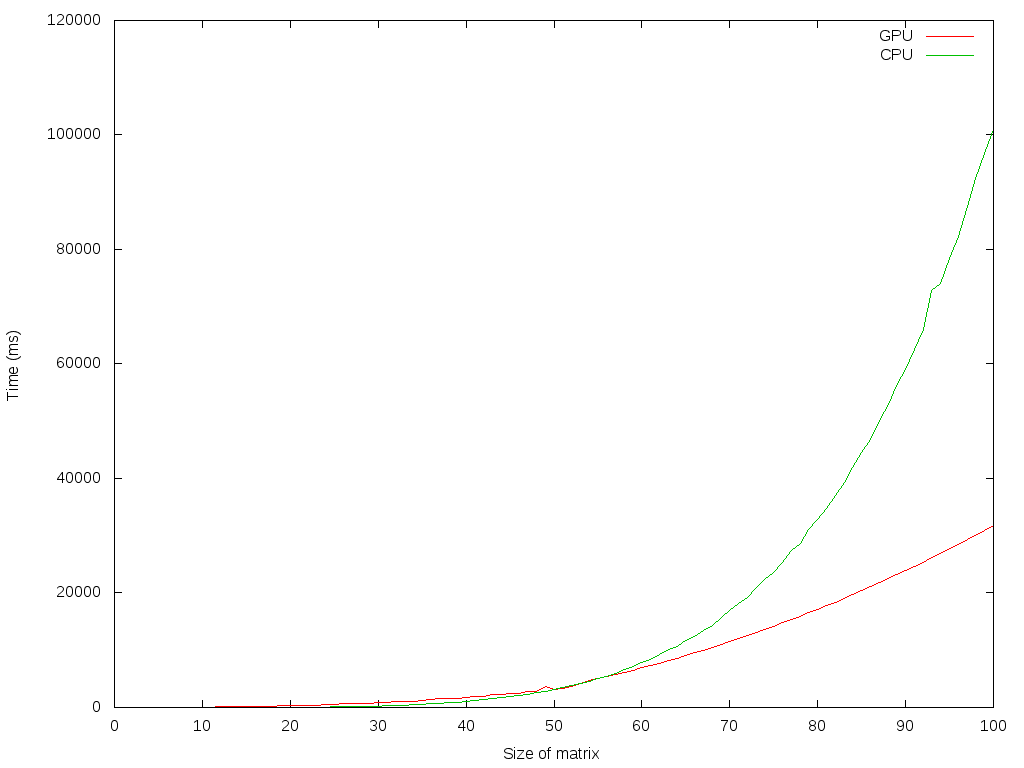
\includegraphics[scale=0.5]{graphic.png}
\end{center}

На графике отчетливо видно, что производительность вычислений на GPU растет с ростом размерности матрицы. На данном примере прослеживается трёхкратное преобладание в скорости работы алгоритма на GPU при размерности задачи N = 100, т.е. матрицы $\mathbb{A}_{100\times100}$

\end{document}